%====================================================================================
\section{The model}
%====================================================================================

\begin{frame}{The model}
	\begin{itemize}
		\item The following model in the first observation:
				\begin{gather}
						y_{i1}=\beta x_{i}+\mu_{i}+\nu_{i1}  \label{model} \\
				  	\intertext{and}
						E\left(\nu _{i1}|x_{i1},\mu_{i}\right) = 0 \notag
				\end{gather} \pause
			\vspace{-.5cm}
		\item Why do we require $\mu_{i}$ to be observed? \pause
				\begin{itemize}
					\item Fixed effects (invariant in time) \pause
					\item Idiosincratic effects. \pause
				\end{itemize}
		\item In the model (\ref{model}) $\beta$ is identified even if we do not observe $\mu_{i}$ but you require that they $(x_{i}$ and $\mu_{i})$ are not correlated:
			\vspace{-.5cm}
				\begin{gather}
					cov\left( x_{i1},\mu _{i}\right) =0 \qquad \beta =\frac{cov\left(x_{i1},y_{i1}\right) }{var\left(x_{i1}\right) }  \label{option1}
				\end{gather} \pause
	\end{itemize}
\end{frame}
%------------------------------------------------
\begin{frame}{Instrumental variables for identification}
		Or the ability to have an instrument
			\begin{align}
				cov\left(Z_{i},\mu_{i}\right) & = 0 \label{option2} \\
				\beta & = \frac{cov\left(Z_{i},y_{i1}\right) }{cov\left(Z_{i},x_{i1}\right)} \notag
			\end{align}
		If $\mu _{i}$ is correlated with $x_{i}?$. So it is true that:
			\begin{eqnarray}
				cov\left(Z_{i},  x_{i}\right) & \neq 0 \notag \\
				cov\left(Z_{i},\mu_{i}\right) & = 0			  \\
				cov\left(Z_{i},\nu_{i}\right) & = 0	   \notag
			\end{eqnarray}
		What we need is the second one for regression strategy to work. we should replace $x_{i}$ with some variable we know is not correlated with $\mu_{i}$ but correlated with $x_{i}$
\end{frame}
%------------------------------------------------
\begin{frame}{We need something else!}
	\begin{itemize}
		\item Suppose that neither of these two above options are available, so a valid strategy is:
				$$y_{i2}=\beta x_{i2}+\mu _{i}+\nu _{i2}$$
			  satisfying
				$$E\left( \nu _{it}|x_{i2},x_{i1},\mu _{i}\right) =0$$
			  taking first differences (difference-in-difference estimator)%
				\begin{gather}
					\beta =\frac{cov\left( \Delta x_{i2},\Delta y_{i2}\right) }{var\left( \Delta x_{i2}\right)}
				\end{gather}
		\item \textbf{Conclusion}: Panel data help us for identifying structural parameters. \pause
	\end{itemize}
\end{frame}

%------------------------------------------------------------------------------------
\subsection{Within-Group estimator}
%------------------------------------------------------------------------------------
\begin{frame}{Within-Group (WG) estimator}
	A simplistic homogeneous model%
		\begin{align}
			y_{it} & =\alpha +X_{it}^{\prime }\beta +u_{it}  \label{earning} \\
			u_{it} & =\mu_{i}+\nu_{it}  \notag
		\end{align}
	heterogeneity given by $\mu _{i}.$\\
	
	Model (\ref{earning}) $y_{it}$ could be a earning equation. So, the dependent variable could be the log of wage. $X$ gathers experience, experience$^{2},$schooling, sex, race, union, marital status and so on., $\mu_{i}$ is the individual specific ability.$\nu_{it}$ is the classical disturbance \emph{iid}. Also, we should take notice that we have the same $\beta$ for all individuals.
\end{frame}
%------------------------------------------------
\begin{frame}{Within-Group (WG) estimator}	
	Arellano (2003) states that the name "withing-group" was originated in the context of data with a group structure. Panel data can be regarded as a special case of this type of data in which the group is formed by the time series observations from a given individual.
\end{frame}
%------------------------------------------------
\begin{frame}{Within-Group estimator and some matrix algebra}
	In order to get the WG estimator we need some matrix algebra. the folowingmodel (another way to present the fixed effects model):
		\begin{align*}
			\underset{NT\times 1}{y} & = \underset{NT\times 1}{\alpha \iota _{NT}}+\underset{NT\times K\text{ }K\times 1}{X\beta }+\underset{NT\times 1}{u} \\
			u & = Z_{\mu }\mu +\nu
		\end{align*}
	where $Z_{\mu}=I_{N}\otimes \iota _{T}.$ $Z_{\mu }$ is a matrix of ones and zeros. Baltagi calls $Z_{\mu}$ the ``matrix of individual dummies''.(\emph{auditorium: we did not get it!}).
\end{frame}
%------------------------------------------------
\begin{frame}{Within-Group estimator and some matrix algebra}
	The matrix $Z_{\mu }$ and for $T=3.$
		$$ Z_{\mu} = \left[	\begin{array}{ccccc}
								1 & 0 & \ldots & 0 & 0 \\ 
								1 & 0 & \ldots & 0 & 0 \\ 
								1 & 0 & \ldots & 0 & 0 \\ 
								0 & 1 & \ldots & 0 & 0 \\ 
								0 & 1 & \ldots & 0 & 0 \\ 
								0 & 1 & \ldots & 0 & 0 \\ 
								\vdots & \vdots & \ddots & \vdots & \vdots \\ 
								0 & 0 & \ldots & 0 & 1 \\ 
								0 & 0 & \ldots & 0 & 1 \\ 
								0 & 0 & \ldots & 0 & 1
				     		\end{array} 
				     \right]$$
\end{frame}
%------------------------------------------------
\begin{frame}{Within-Group estimator and some matrix algebra}
	some curiosities (it is worth getting them!):%
		\begin{gather}
			Z_{\mu }Z_{\mu }^{\prime }=I_{N}\otimes J_{T}  \label{curiosity1}
		\end{gather}
	where $J_{T}$ is a matrix of ones of dimension T. How did you get expression $\left( \ref{curiosity1}\right)$?.
		\begin{align*}
			Z_{\mu }Z_{\mu }^{\prime } &= \left( I_{N}\otimes \iota _{T}\right) \left(
			I_{N}\otimes \iota _{T}\right) ^{\prime } \\
			Z_{\mu }Z_{\mu }^{\prime } &= I_{N}\otimes \iota _{T}\iota _{T}^{\prime } \\
			Z_{\mu }Z_{\mu }^{\prime } &= I_{N}\otimes J_{T}
		\end{align*}
	(\emph{auditorium: Fred, why you are showing this? where are we going to?})
\end{frame}
%------------------------------------------------
\begin{frame}{Within-Group estimator and some matrix algebra}
	a new matrix (an idempotent one!):
		$$P_{\mu }=Z_{\mu }\left( Z_{\mu }^{\prime }Z_{\mu }\right) ^{-1}Z_{\mu}^{\prime }$$
	P is an inetersting matrix because if you pre multiply this matrix with a row vector, you will have a vector of meaned series across time. (\emph{ auditorium: How do you get this result?}). Let's see, we know that
		\begin{align*}
			Z_{\mu}^{\prime}Z_{\mu} & = \left(I_{N}\otimes \iota_{T}^{\prime}\right) \left(I_{N}\otimes \iota_{T}\right) \\
			Z_{\mu}^{\prime}Z_{\mu} & = I_{N}\otimes T \\
			Z_{\mu}^{\prime}Z_{\mu} & = T\cdot I_{N}
		\end{align*}
\end{frame}
%------------------------------------------------
\begin{frame}{Within-Group estimator and some matrix algebra}	
	considering expression for $P_{\mu }$ (projection matrix on $Z_{\mu }$) and incorporating on it the above results: 
		\begin{align*}
			P & = T^{-1}\left(I_{N}\otimes J_{T}\right) \\
			P & = I_{N}\otimes \overline{J}_{T}
		\end{align*}
	where $\overline{J}_{T} = J_{T} \cdot T^{-1}.$ So, it is clear that
		\begin{itemize}
			\item $\underset{NT\times 1}{Py}$ which has a typical element $\overline{y}_{i}=T^{-1}\sum_{t=1}^{T}y_{it}$ \pause
			\item $\underset{NT\times 1}{Qy}$ which has a typical element $\widetilde{y}_{it}=y_{it}-T^{-1}\sum_{t=1}^{T}y_{it}.$ $Q=I-P_{\mu}.$
		\end{itemize}
\end{frame}
%------------------------------------------------
\begin{frame}{Within-Group estimator}
	the matrix $\underset{NT\times NT}{Q}$ is known as the deviations-from time-means or withing group estimator because it transforms the originals eries into deviations from time means
		$$\widetilde{y}_{i}=Qy_{i}$$
	again $\underset{NT\times 1}{Qy}$ which has a typical element $\widetilde{y}_{i}=y_{it}-T^{-1}\sum_{t=1}^{T}y_{it}.$ $Q=I-P_{\mu }.$
	    \begin{block}{Some properties}
			\begin{center}
				$P+$Q=$I$ \\
				$P,$Q idempotent $P$P=$P,\, $Q $Q$=Q \\
				and $P$Q=0
			\end{center}
		\end{block}
\end{frame}
%------------------------------------------------
\begin{frame}{Within-Group estimator}
	Considering the model:
		\begin{align*}
			\underset{NT\times 1}{y} & = \underset{NT\times 1}{\alpha \iota _{NT}}+\underset{NT\times K\text{ }K\times 1}{X\beta }+\underset{NT\times 1}{u} \\
			u & =Z_{\mu }\mu +\nu
		\end{align*}
	$Z_{\mu }$ is the ``matrix of individual dummies'',$\mu $ is a $N\times 1$ column vector. Setting up the transformation:
		$$Qy=QX\beta +Q\nu$$
	the estimator withing group (recall econometric review session) 
		$$\widehat{\beta}_{WG}=\left(X^{\prime }QX\right)^{-1}\left(X^{\prime}Qy\right)$$
\end{frame}
%------------------------------------------------
\begin{frame}{Within-Group estimator}
	the estimator withing group:
		\begin{gather}
			\widehat{\beta}_{WG}=\left(X^{\prime }QX\right)^{-1}\left(X^{\prime}Qy\right) \label{within-group}
		\end{gather}
	the individual effects are wiped out. Vector $\beta_{WG}$ gathers parameters of interest, incidental parameters are not included because they are individual effects. Expression (\ref{within-group}) is the withing-group or fixed effects estimator This estimator is very popular and most of econometric softwares have implement it. STATA and Eviews do this procedure and they construct the dummies series (for each member of panel) but they do not show the dummies.
\end{frame}
%------------------------------------------------
\begin{frame}{Within-Group estimator}
	we need an estimate of $V$
		$$\widehat{V}=\frac{1}{N}\widetilde{X}^{\prime }\widehat{\Xi }\text{ } \widetilde{X}$$
	where
$$\widehat{\Xi }=\left[ 
		\begin{array}{cccc}
			\underset{\left( T\times 1\right) \left( 1\times T\right) }{\widehat{\nu }%
				_{1\cdot }\widehat{v}_{1\cdot }^{\prime }} & \mathbf{0} & \cdot & \mathbf{0}
			\\ 
			\mathbf{0} & \underset{\left( T\times 1\right) \left( 1\times T\right) }{%
				\widehat{\nu }_{2\cdot }\widehat{v}_{2\cdot }^{\prime }} & \cdot & \mathbf{0}
			\\ 
			\cdot & \cdot & \cdot & \cdot \\ 
			\mathbf{0} & \mathbf{0} & \cdot & \underset{\left( T\times 1\right) \left(
				1\times T\right) }{\widehat{\nu }_{N\cdot }\widehat{v}_{N\cdot }^{\prime }}%
		\end{array}
\right]_{\dim \, NT\times NT}$$
	where $\widehat{\nu}_{i}=\widetilde{y}_{i}-\widetilde{X}_{i}\widehat{\beta}$
\end{frame}
%------------------------------------------------
\begin{frame}{Within-Group estimator}
	\begin{center}
		\Huge{Let's go to Excel!}
	\end{center}
\end{frame}
%------------------------------------------------
\begin{frame}{Within-Group estimator}
	In Arellano's terms
		\begin{align*}
			\widehat{\beta }_{WG}  = & \left[ \sum_{i=1}^{N}\sum_{t=1}^{T}\left( x_{it}-%
			\overline{x}_{i}\right) \left( x_{it}-\overline{x}_{i}\right) ^{\prime }%
			\right] ^{-1} \\
			& \left[ \sum_{i=1}^{N}\sum_{t=1}^{T}\left( x_{it}-\overline{x}_{i}\right)
			\left( y_{it}-\overline{y}_{i}\right) ^{\prime }\right]
		\end{align*}
\end{frame}
%------------------------------------------------
\begin{frame}{Within-Group estimator Vs. OLS}
	Biased and inconsistency parameters under a true model.
		\begin{center}
			\begin{tikzpicture}
	\begin{axis}[samples=100,
				 xmin = 0, xmax = 8,
				 ymin = 0, ymax = 10,
				 axis lines* = left,
				 xtick = \empty, ytick = \empty,
				 clip = false,
				 xmajorgrids=true, ymajorgrids=true]
		
		% Lines
		\addplot [ ] coordinates {(0, 2) (6, 4)};
		\addplot [ ] coordinates {(0, 4) (7, 6.33)};
		\addplot [ ] coordinates {(0, 6) (8, 8.67)};
		\addplot [ ] coordinates {(2, 0) (5, 10)};
		
		% Points
		\addplot[smooth,thick,mark=x] coordinates {(3.51, 2.56)};
		\addplot[smooth,thick,mark=x] coordinates {(3.58,3.54)};
		\addplot[smooth,thick,mark=x] coordinates {(2.17,3.14)};
		\addplot[smooth,thick,mark=x] coordinates {(2.66,3.95)};
		\addplot[smooth,thick,mark=x] coordinates {(2.71,4.58)};
		\addplot[smooth,thick,mark=x] coordinates {(3.84,4.21)};
		\addplot[smooth,thick,mark=x] coordinates {(4.51,4.56)};
		\addplot[smooth,thick,mark=x] coordinates {(3.84,4.95)};
		\addplot[smooth,thick,mark=x] coordinates {(4.58,5.37)};
		\addplot[smooth,thick,mark=x] coordinates {(4,6)};
		\addplot[smooth,thick,mark=x] coordinates {(4.41,7.02)};
		\addplot[smooth,thick,mark=x] coordinates {(1.59,4.95)};
		\addplot[smooth,thick,mark=x] coordinates {(2.36,5.23)};
		\addplot[smooth,thick,mark=x] coordinates {(3.04,5.84)};
		\addplot[smooth,thick,mark=x] coordinates {(2.64,6.15)};
		\addplot[smooth,thick,mark=x] coordinates {(3.33,6.79)};
		
		% Labels
		\node [left]  at (0, 20)  {alfa 1};
		\node [left]  at (0, 40)  {alfa 2};
		\node [left]  at (0, 60)  {alfa 3};
		\node [right] at (500,100)  {OLS};
		
	\end{axis}
\end{tikzpicture}
		\end{center}
\end{frame}
%------------------------------------------------
\begin{frame}{Within-Group estimator is not a Panacea}
	(Real) heterogeneity in panel data
		\begin{center}
			\begin{tikzpicture}
	\begin{axis}[samples=100,
		xmin = 0, xmax = 8,
		ymin = 0, ymax = 10,
		axis lines* = left,
		xtick = \empty, ytick = \empty,
		clip = false,
		xmajorgrids=true, ymajorgrids=true]
		
		% Lines
		\addplot [dashed] coordinates {(0.5, 3) (9, 5.5)};
		\addplot [] coordinates {(0.7, 2.5) (3, 5)};
		\addplot [] coordinates {(3,2.8) (4, 6.5)};
		\addplot [] coordinates {(4.2,5.5) (5, 2.5)};
		\addplot [] coordinates {(5.7,2.9) (8.5,6.8)};
		
		% Labels
		\node [below]  at (90,25)   {\small $i=1$};
		\node [below]  at (360, 27) {\small $i=2$};
		\node [right]  at (440, 55) {\small $i=3$};
		\node [below]  at (600,25)  {\small $i=4$};
		\node [below]  at (900,50)  {OLS};
		
	\end{axis}
\end{tikzpicture}
		\end{center}
\end{frame}
%------------------------------------------------
\begin{frame}{Within-Group estimator's disadvantages}
	\begin{itemize}
		\item N-1 dummies for those fixed effects. A lof of degrees of freedom lost but people like and want to see dummies.
		\item ``\emph{I wanted to see the dummy for year 2006, but I couldn't!}''. Stata randomly drops one or more dummies if there is perfect collinearity.
		\item A lot of dummies vs a procedure which estimates just 1 parameter.
		\item the procedure wipes out individual time-invariant specifical variables which maybe we are interested (in earning equations variables as sex, race and religion and so on are important).
	\end{itemize}
\end{frame}
%------------------------------------------------
\begin{frame}{Within-Group estimator's advantages}
	\begin{itemize}
		\item In terms of specification: OLS baised and inconsistent if within-group effects are important (omitted variables problem).
		\item Specifical variables are already interesting in our study (in earning equations variables as sex, race and religion and so on are important). But that is not a problem if we deal with LSDV (least squares dummy variables).
	\end{itemize}
\end{frame}
%------------------------------------------------
\begin{frame}{Within-Group estimator's Interpretation}
	\begin{itemize}
		\item $\mu_{i}$ are fixed $($Baltagi ``\emph{or random but hopelessly correlated with }$\mathit{X}_{it}'')$
		\item In other words if the true model does have fixed effects so OLS is biased and inconsistent.
	\end{itemize}
\end{frame}
%------------------------------------------------
\begin{frame}{Within-Group STATA syntax}
	in Stata syntax:
		$$\colorbox{codegray}{\text{\texttt{xtreg \textit{depvar} [\textit{indepvars}] [if] [in] [, fe \textit{FE\_options}]}}}$$	
	an example for variables \colorbox{codegray}{\texttt{Y1 X1 X2}} and group identifier \colorbox{codegray}{\texttt{varname}}
		$$\colorbox{codegray}{\textcolor{codeblue}{xtreg} Y1 X1 X2, fe}$$
	before you perform \colorbox{codegray}{\textcolor{codeblue}{\texttt{xtreg}}} you should set up the panel structure, use \colorbox{codegray}{\texttt{xtsset}}.\\
		\medskip
	See \colorbox{codegray}{\textcolor{codeblue}{\texttt{help xtreg}.}}
\end{frame}
%------------------------------------------------
\begin{frame}{Within-Group STATA syntax}
	\begin{figure}
		\centering
			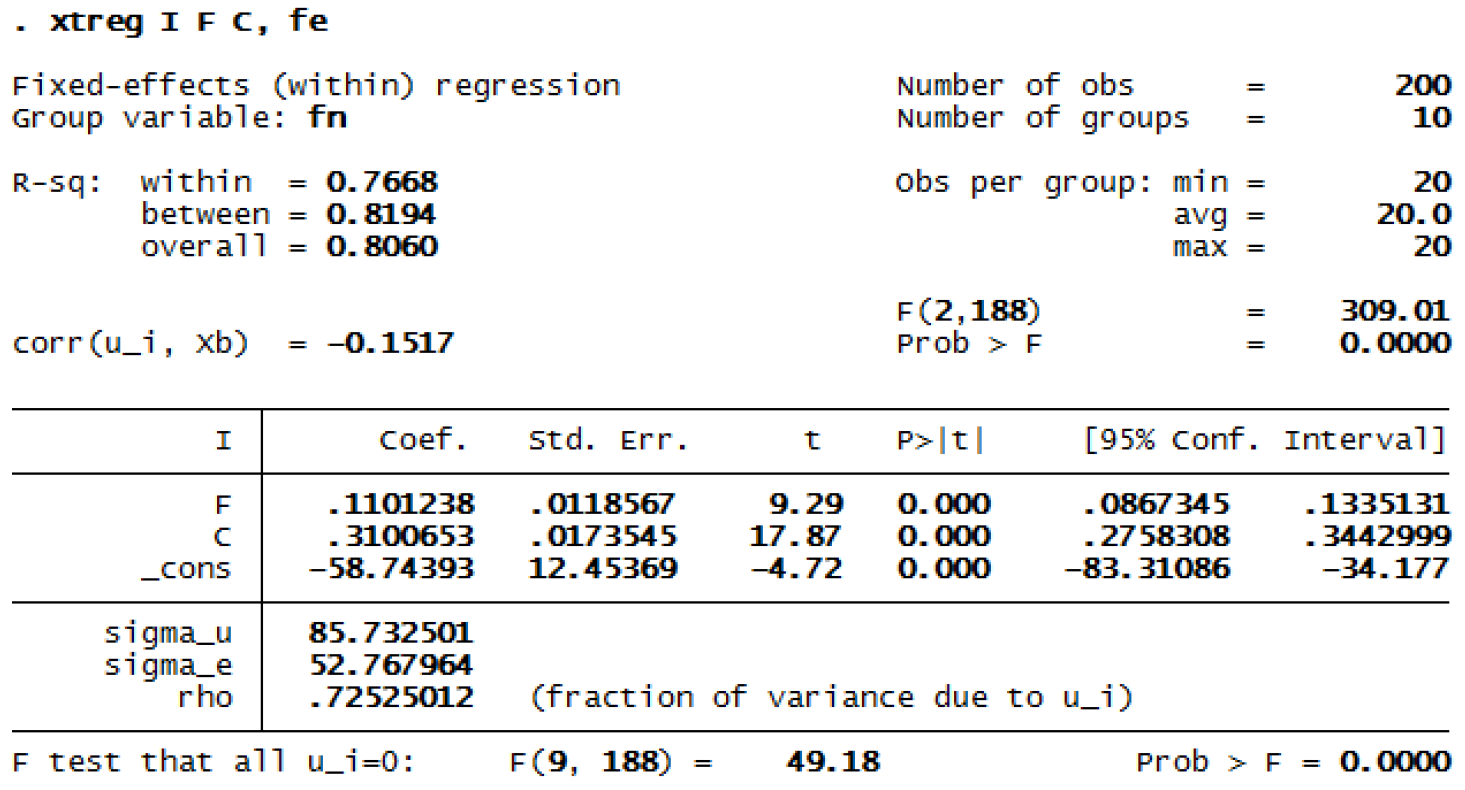
\includegraphics[width = 0.9\linewidth]{figures/panel_01.png}
	\end{figure}
\end{frame}
%------------------------------------------------
\begin{frame}{Within-Group STATA output}
	\begin{itemize}
		\item At the top of the output we can see an ``\textit{overall}'' F\ test but this includes only of those terms ``we are interested'' (excluding incidental parameters).
		\item There is a F-test under the null: all $\mu _{i}=0.$
		\item $rho=\frac{\sigma_{\mu }^{2}}{\sigma_{\mu}^{2}+\sigma_{\nu}^{2}}$
		\item The output shows the unrestricted correlation between $\mu_{i}$ and $X\prime s.$
		\item Under this command \texttt{xtreg} the dummies (fixed effects) are not shown.
	\end{itemize}
\end{frame}
%------------------------------------------------
\begin{frame}{FE options}
	\begin{figure}
		\centering
			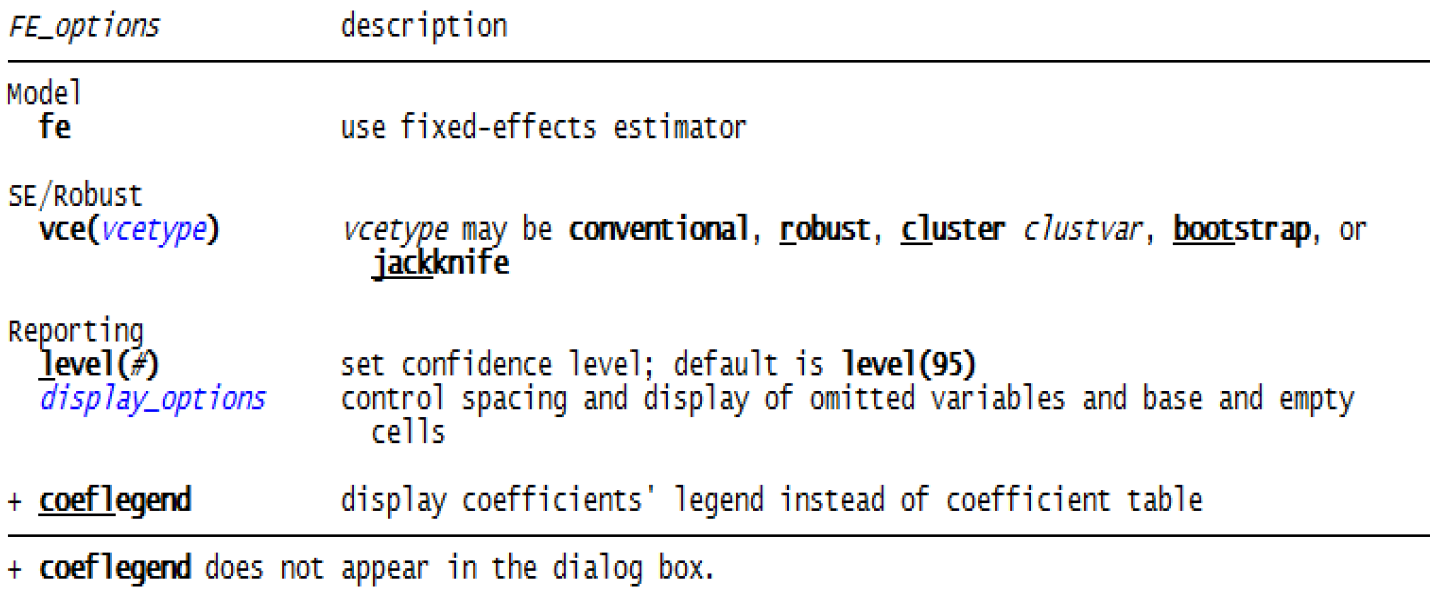
\includegraphics[width = 0.9\linewidth]{figures/panel_02.png}
	\end{figure}
\end{frame}
%------------------------------------------------
\begin{frame}{Within-Group STATA}
	Other way to estimate fixed effects
		$$\colorbox{codegray}{areg depvar [\textit{indepvars}] [if] [in] ,a(\textit{varname}) [options]}$$
	an example for variables \texttt{Y1 X1 X2} and group identifier \texttt{varname}
		$$\colorbox{codegray}{\texttt{\textcolor{codeblue}{areg} Y1 X1 X2, a(id)}}$$
	See \colorbox{codegray}{\textcolor{codeblue}{\texttt{h areg}}}. This \emph{absorb} command is useful because you also have an overall F test including the dummies variables
\end{frame}
%------------------------------------------------
\begin{frame}{Options}
	\colorbox{codegray}{\textcolor{codeblue}{\texttt{areg}}}
		\begin{figure}
			\centering
			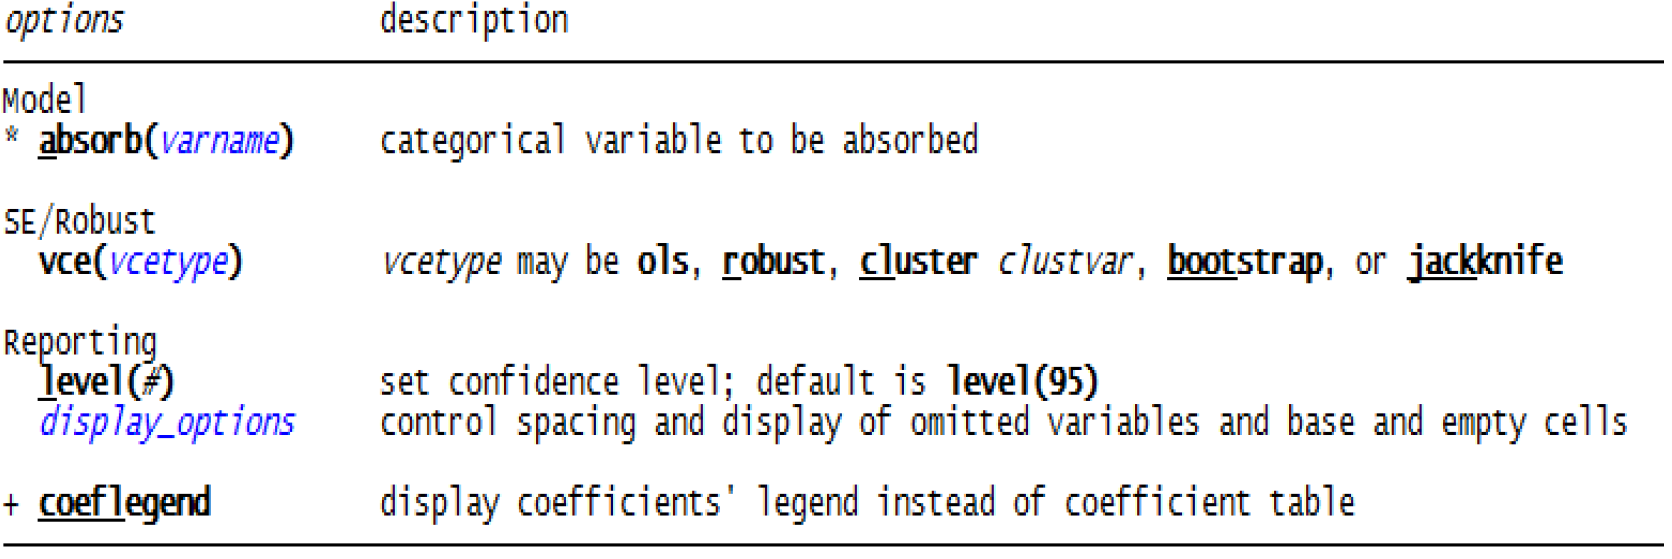
\includegraphics[width = 0.9\linewidth]{figures/panel_03.png}
		\end{figure}
\end{frame}
%------------------------------------------------
\begin{frame}{Output}
	\colorbox{codegray}{\textcolor{codeblue}{\texttt{areg}}}
		\begin{figure}
			\centering
			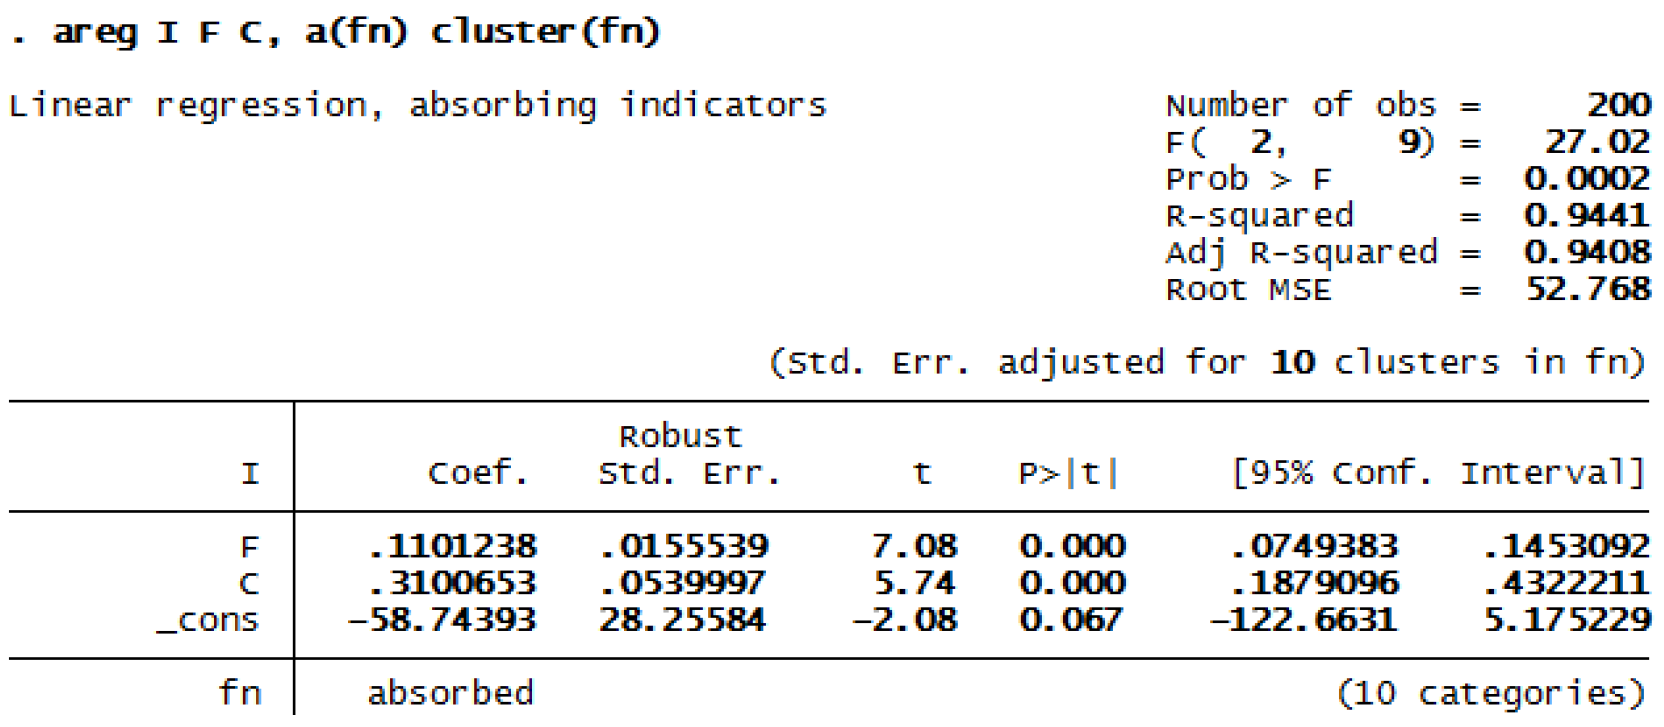
\includegraphics[width = 0.9\linewidth]{figures/panel_04.png}
		\end{figure}
\end{frame}
%------------------------------------------------
\begin{frame}{Least squares dummy variables (LSDV)}
	Incorporating the dummies in the X matrix and perform:%
		\begin{gather}
			\widehat{\beta}_{LSDV}=\left(X^{+\prime}X^{+}\right) ^{-1}\left(X^{+\prime }y^{+}\right)
		\end{gather}
	where $X^{+}=\left[ X\quad I_{N}\otimes \iota _{T}\right] .$ In Stata syntax:
		$$\colorbox{codegray}{\texttt{xi [, prefix(\textit{string})noomit] i. varname}}$$
	an example for variables \colorbox{codegray}{\texttt{Y1 X1 X2}} and group identifier \colorbox{codegray}{\texttt{varname}}
		\begin{exampleblock}{STATA code}
			\centering
			\texttt{\textcolor{codeblue}{xi}: \textcolor{codeblue}{reg} Y1 X1 X2, i.varname}
		\end{exampleblock}
\end{frame}
%------------------------------------------------
\begin{frame}{Least squares dummy variables (LSDV)}
	Other way to get the dummies into the regresion.\\
	In Stata syntax:
		\begin{eqnarray*}
			&&\cdot \text{[\texttt{quietly] tab \textit{varname}, [gen(\textit{stubname}%
					)]}} \\
			&&\cdot \text{\texttt{reg depvar [\textit{indepvar}] \textit{stubname*}[if]
					[in] [,\textit{options}]}}
		\end{eqnarray*}%
	an example for variables \colorbox{codegray}{\texttt{Y1 X1 X2}} and group identifier \colorbox{codegray}{\texttt{varname}}
	    \begin{exampleblock}{STATA code}
	    	\centering
	    		\texttt{\textcolor{codeblue}{quietly tab} id, gen(dum)}\\
	    		\hspace{-1.65cm} \texttt{\textcolor{codeblue}{reg} Y1 X1 X2 dum*}
		\end{exampleblock}
\end{frame}
%------------------------------------------------
\begin{frame}{Let's go to STATA}
	Let's go to STATA. Please, Download data from \colorbox{codegray}{\texttt{\textcolor{codecrimson}{\textquotedbl www.wiley.co.uk/baltagi\textquotedbl}}}. Definition of variables is as follows
		\begin{itemize}
			\item $I_{it}$ denotes real gross investment for firm $i$ in year $t.$
			\item $F_{it}$ is the real value of the firm (shares outstanding).
			\item $C_{it}$ is the real value of the capital stock.
		\end{itemize}
	10 large US\ manufacturing firms over 20 years 1935-54.
\end{frame}
%------------------------------------------------
\begin{frame}{Within-Group estimator}
	therefore, the robust asymptotic variance and covariance matrix of $\beta$ is estimated by:
		\begin{align}
			var\left( \beta \right) & = \frac{1}{N}\cdot \left( \widetilde{\mathbf{X}}%
			^{\prime }\widetilde{\mathbf{X}}\right) ^{-1}N\cdot \left( \frac{1}{N}%
			\widetilde{\mathbf{X}}^{\prime }\widehat{\Xi }\text{ }\widetilde{\mathbf{X}}%
			\right) \cdot \left( \widetilde{\mathbf{X}}^{\prime }\widetilde{\mathbf{X}}%
			\right) ^{-1}N  \notag \\
			var\left( \beta \right) & = \left( \widetilde{\mathbf{X}}^{\prime }\widetilde{%
				\mathbf{X}}\right) ^{-1}\cdot \left( \widetilde{\mathbf{X}}^{\prime }%
			\widehat{\Xi }\text{ }\widetilde{\mathbf{X}}\right) \cdot \left( \widetilde{%
				\mathbf{X}}^{\prime }\widetilde{\mathbf{X}}\right) ^{-1}
		\end{align}
	if $\widehat{\Xi }$ $=\sigma ^{2}I_{NT}$ so:
		$$var\left( \beta \right) =\sigma ^{2}\left( \widetilde{\mathbf{X}}^{\prime }\widetilde{\mathbf{X}}\right) ^{-1}$$
\end{frame}
%------------------------------------------------
\begin{frame}{Within-Group estimator, summarizing...}
	\begin{itemize}
		\item OLS\ biased and inconsistent when the true model is a FE model. Baltagi states this result is because of an ``omitted variables problem''.
		\item Test for individual dummies (standard F test). Useful for testing Pooling models.
		\item Test using LR test (imposing restrictions).
		\item Robust Standard Errors (Arellano;1987).
	\end{itemize}
\end{frame}
%------------------------------------------------
\begin{frame}{Alternative estimator for fixed effects: difference in difference}
	\begin{itemize}
		\item Withing group estimator is not the only transformation that will drop out the individual effects.
		\item Difference-indifference estimator makes the trick as well.
		\item Strategy of information only estimates parameters of "interest".
	\end{itemize}
\end{frame}
%------------------------------------------------
\begin{frame}{Alternative estimator for fixed effects: difference in difference}
	Which in compact form can be written as
		$$Dy_{i}=DX_{i}\beta +D\nu _{i}$$
	where D is the $\left( T-1\right) \times T$ matrix ``first-difference operator''
		$$D=\left[ \begin{array}{cccccc}
						-1 & 1 & 0 & \cdots & 0 & 0 \\ 
						0 & -1 & 1 & \cdots & 0 & 0 \\ 
						\vdots & \vdots & \vdots & \ddots & \vdots & \vdots \\ 
						0 & 0 & 0 & \cdots & -1 & 1
					\end{array}
			\right]$$
	under assumptions $E\left( D\nu_{i}|x_{i}\right) = 0$ and/or $E\left( D\nu_{i}|x_{i}\right) =0$ (Arellano; 2003)$,$
\end{frame}
%------------------------------------------------
\begin{frame}{Alternative estimator for fixed effects: difference in difference}
	In terms of panel structure
		$$\underset{\dim N\times T-1}{D_{N}}=I_{N}\otimes D$$
	thus pre-multiplying this matrix to data
\end{frame}
%------------------------------------------------
\begin{frame}{Alternative estimator for fixed effects: difference in difference}
	OLS estimates of $\beta $ in this system given by
		$$\widehat{\beta}_{D}=\left(\left(D_{N}X\right)^{\prime}\left(D_{N}X\right) \right) ^{-1}\left(\left(D_{N}X\right)^{\prime}\left(D_{N}y\right) \right)$$
	Arellano (2003) considers
		$$\widehat{\beta}_{D}=\left(\sum_{i=1}^{N}\left(X_{i}^{\prime }D^{\prime}DX_{i}\right) \right)^{-1}\sum_{i=1}^{N}\left(DX_{i}\right)^{\prime}\left(Dy_{i}\right)$$
	this $\widehat{\beta}_{D}$ is unbiased and consistent for large $N$. What about the variance?
\end{frame}
%------------------------------------------------
\begin{frame}{Alternative estimator for fixed effects: difference in difference}
	the variance matrix of errors
		$$var\left(D_{N}\nu|X\right)=\left(\sigma_{\nu }^{2}I_{NT}\right) \cdot D_{N}D_{N}^{\prime}$$
	which show an autocorrelation structure%
		$$var\left( D_{N}\nu |X\right) =\left[ 
				\begin{array}{cccccc}
					2\sigma _{\nu }^{2} & 0 & 0 & \ldots & 0 & 0 \\ 
					-\sigma _{\nu }^{2} & 2\sigma _{\nu }^{2} & 0 & \ldots & 0 & 0 \\ 
					0 & -\sigma _{\nu }^{2} & 2\sigma _{\nu }^{2} & \ldots & 0 & 0 \\ 
					\vdots & \vdots & \vdots & \ddots & \vdots & 0 \\ 
					0 & 0 & 0 & \ldots & -\sigma _{\nu }^{2} & 2\sigma _{\nu }^{2}
				\end{array}
			  \right]$$
	result: difference in difference estimator is not BLUE because it is inefficient (but unbiased). That means that Gauss Markov theorem is not hold.
\end{frame}
%------------------------------------------------
\begin{frame}{Alternative estimator for fixed effects: difference in difference}
	\textbf{Solution: generalized squares}. Following the standard procedure we should use GLS. This matrix makes the trick:
		$$P_{D_{N}}=D_{N}^{\prime }\left( D_{N}^{\prime }D_{N}\right) ^{-1}D_{N}$$
	$P_{D_{N}}$ is idempotent $P_{D_{N}}P_{D_{N}}^{\prime }=P_{D_{N}}$ or $P_{D_{N}}P_{D_{N}}=P_{D_{N}}.$ So,
		$$\widehat{\beta }_{WG}=\left( \sum_{i=1}^{N}\left( X_{i}^{\prime
		}P_{D_{N}}X_{i}\right) \right) ^{-1}\sum_{i=1}^{N}X_{i}^{\prime
		}P_{D_{N}}y_{i}$$
\end{frame}
%------------------------------------------------
\begin{frame}{Alternative estimator for fixed effects: difference in difference}
	such a nice surprise!. The idempotent matrix $P_{D_{N}}$ also takes the form:
		$$P_{D_{N}}=I_{NT}-I_{N}\otimes \overline{J}_{T}=Q$$
	So, the difference in difference estimator is unbiased and consistent.
\end{frame}
%------------------------------------------------
\begin{frame}{Alternative estimator for fixed effects: difference in difference}
	\textbf{Orthogonal deviations}. Finally, we have realized that if we are using difference and difference we need to do 2 transformations: a) to get differenced data and b) remove the moving-average serial correlation (known pattern) induced by a). The overall tranformation is:
		$$A=\left( D_{N}D_{N}^{\prime }\right) ^{-\frac{1}{2}}D_{N}$$
	therefore $\nu ^{\ast }=A\nu $ which will have $T-1$ elements by $i$
		\begin{align*}
			s_{it}^{\ast } & = c_{t}\cdot \left[s_{it}-\frac{1}{T-t}\left(s_{it+1}+...+s_{iT}\right) \right] \text{ } \\
			t & = 1,...,T-1
		\end{align*}
\end{frame}
%------------------------------------------------
\begin{frame}{Alternative estimator for fixed effects: difference in difference}
	where $c_{t}=\left( \frac{T-t}{T=t-1}\right)^{\frac{1}{2}}.$(see Arellano and Bover; 1995). thus, we get for each first ($T-1$) observations we substract the mean of the remaining future observations in the sample. The weighting $c_{t}$ is introduced because variances of transformed erros must be equalized. This transformation is called ``\emph{forward orthogonal deviations}''.
\end{frame}
%------------------------------------------------
\begin{frame}{Difference in difference estimator: summarizing...}
	\begin{itemize}
		\item FE is more efficient than difference in difference (FD) estimator when  $\nu_{it}$ are \emph{iid}.
		\item FD is more efficient than FE estimator when $\nu_{it}$ is random walk.
		\item Both estimators are affected in different ways when there are measurements errors.
	\end{itemize}
\end{frame}
%------------------------------------------------
\begin{frame}{Efficiency of difference-in-difference estimator}
	\begin{itemize}
		\item FD is more efficient than FE estimator when $\nu_{it}$ is random walk $\left( \nu_{it}=\nu_{it-1}+\xi_{it}\right) $. Recalling that
			\begin{align*}
				var\left( D_{N}\nu |X\right) & = D_{N}vv^{\prime }D_{N}^{\prime } \\
											 & = \xi \xi ^{\prime } \\
											 & = \sigma _{\xi }^{2}\cdot I_{NT}
			\end{align*}
	\end{itemize}
\end{frame}

%------------------------------------------------------------------------------------
\subsection{Between-Group estimator}
%------------------------------------------------------------------------------------

\begin{frame}{Between-Group estimator}
		\begin{itemize}
			\item This estimator between group can be derived using the projection matrix $P$
					\begin{align*}
						\underset{NT\times 1}{y} & = \underset{NT\times 1}{\alpha \iota 
													 _{NT}}+\underset{NT\times K\text{ }K\times 1}{X\beta }+\underset{NT\times 1}{u} \\
											   u & = Z_{\mu }\mu +\nu
					\end{align*}
		\end{itemize}
	premultiplying by P
		\begin{gather}
			Py=P\iota _{NT}+PX\beta +Pu  \label{BE0}
		\end{gather}
	the LS estimator under (\ref{BE0}). (Recall econometric review session)
		\begin{gather}
			\beta_{BE}=\left( X^{\prime }\left( P-\overline{J}_{NT}\right) X\right)^{-1}\left( X^{\prime}\left( P-\overline{J}_{NT}\right) y\right)
		\end{gather}
\end{frame}
%------------------------------------------------
\begin{frame}{Between-Group estimator}
	\begin{itemize}
		\item The estimator between group (in easy format):
			\begin{gather}
				\overline{y}_{i}=\alpha +\overline{X}_{i}\beta +\overline{u}_{i}  \label{BE}
			\end{gather}
		the cross-section regression is based on N observations. The STATA syntax is
			$$\colorbox{codegray}{\texttt{xtreg \textit{depvar} [\textit{indepvars}] [if] [in] [,be \textit{BE\_options}]}}$$
		an example for variables \colorbox{codegray}{\texttt{Y1 X1 X2}} and group identifier \colorbox{codegray}{\texttt{varname}}
	\end{itemize}
\end{frame}
%------------------------------------------------
\begin{frame}{BE options}
	\begin{figure}
		\centering
		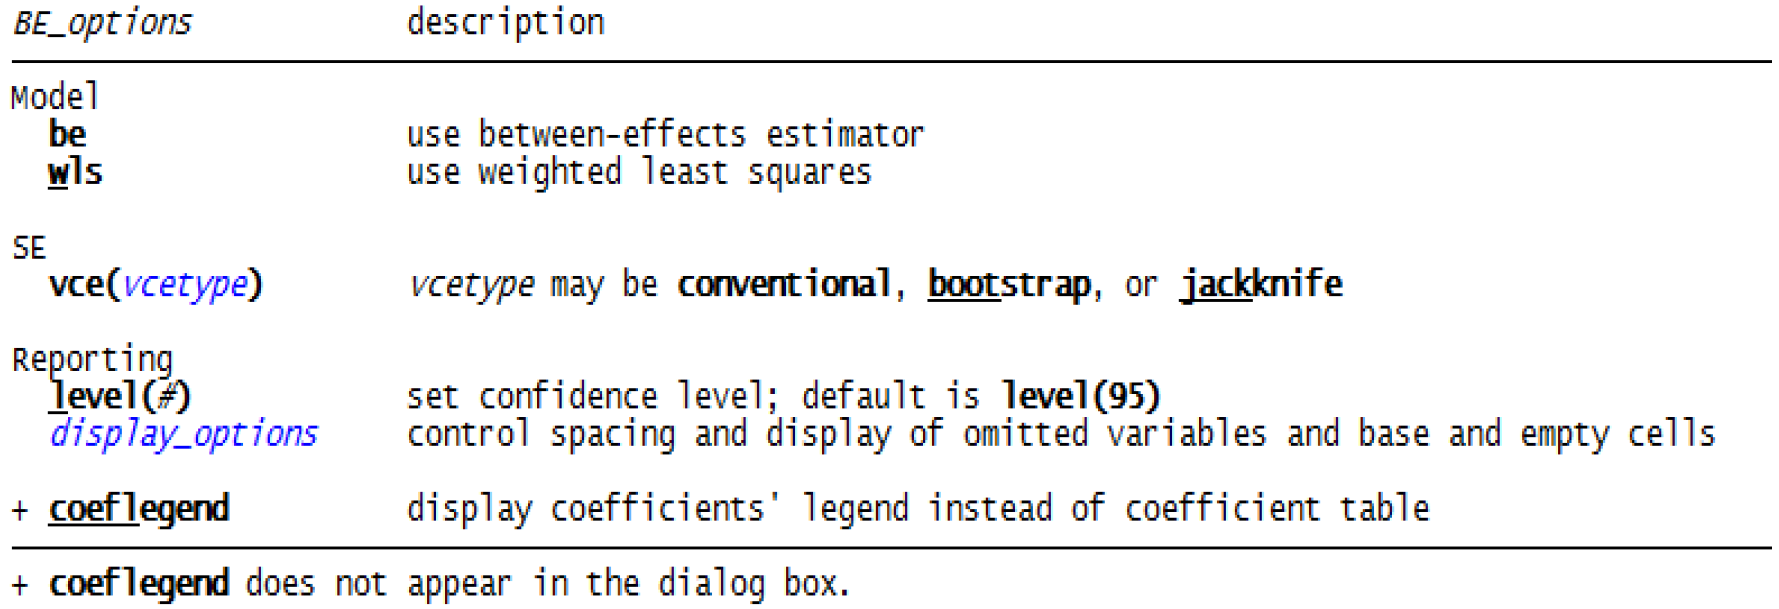
\includegraphics[width = \linewidth]{figures/panel_05.png}
	\end{figure}
\end{frame}
%------------------------------------------------
\begin{frame}{BE-estimator output}
	\begin{figure}
		\centering
		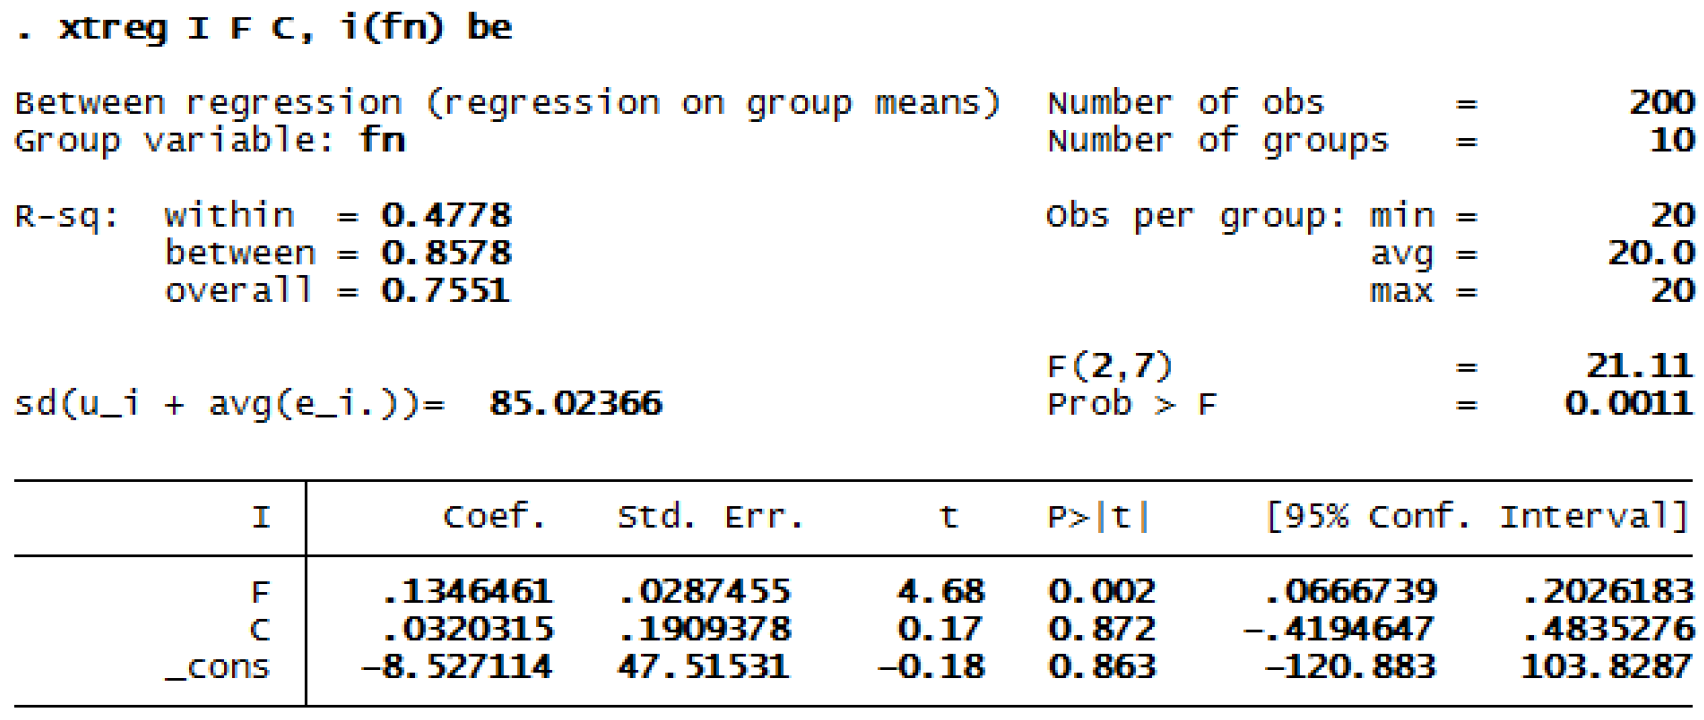
\includegraphics[width = \linewidth]{figures/panel_06.png}
	\end{figure}
\end{frame}

%------------------------------------------------------------------------------------
\subsection{Random Efects model}
%------------------------------------------------------------------------------------

\begin{frame}{Random Effect model}
	\begin{itemize}
		\item Baltagi states that within-group estimation would mean a loss of degrees of freedom. That statement comes from the fact that within-group estimator needs to estimate $N$ fixed effects or include $(N-1)$ dummies as regresors. \pause
		\item In this especification the individual effect is characterized as random and drawn from a sample, inference is conducted using that sample. \pause
		\item Nerlove and Balestra (1996)'s estimator. \pause
		\item Haavelmo (1944).
	\end{itemize}
\end{frame}
%------------------------------------------------
\begin{frame}{Random Effect model}
	A simplistic homogeneous model
		\begin{align}
			y_{it} & = \alpha +X_{it}^{\prime }\beta +u_{it} \\
			u_{it} & = \mu _{i}+\nu _{it}  \notag
		\end{align}
	heterogeneity given by $\mu _{i}.$ $\mu _{i}\backsim N\left( 0,\sigma _{\mu
	}^{2}\right) $ and $\nu _{it}\backsim N\left( 0,\sigma _{\nu }^{2}\right) .$
		\begin{align*}
			u_{it}u_{it}^{\prime } & = \left( \mu _{i}+\nu _{it}\right) \left( \mu
										_{i}+\nu _{it}\right) ^{\prime } \\
			\sigma ^{2} & = \sigma _{\mu }^{2}+\sigma _{\nu }^{2}
		\end{align*}%
	$\sigma ^{2}$ is the variance \ based in the latter we construct $\rho = \frac{\sigma _{\mu }^{2}}{\sigma ^{2}}$ (\emph{equicorrelation}).
\end{frame}
%------------------------------------------------
\begin{frame}{Random Effect model}
	the error component for $it$
		$$u_{it}=\mu _{i}+\nu _{it}$$
	the error component for all (matrix form)%
		$$u=\left( I_{N}\otimes \iota _{T}\right) \mu +\nu$$
	we need to have the total (expected) variance of the error component%
		\begin{align*}
			u^{\prime }u & = \mu ^{\prime }\left( I_{N}\otimes \iota _{T}\right) ^{\prime
							 }\left( I_{N}\otimes \iota _{T}\right) \mu +\nu ^{\prime }v \\
						 & = \mu ^{\prime }\left( I_{N}\otimes \iota _{T}^{\prime }\iota _{T}\right)
							 \mu +\nu ^{\prime }v
		\end{align*}
	Taking expectations
		\begin{gather}
			E(u^{\prime }u)=T\sigma _{\mu }^{2}+\sigma _{\nu }^{2}
		\end{gather}
\end{frame}
%------------------------------------------------
\begin{frame}{Random Effect model}
	getting the ``verall'' matrix variance%
		$$u=\left( I_{N}\otimes \iota _{T}\right) \mu +\nu$$
	So,
		\begin{align*}
			\underset{NT\times NT}{\Omega } & = E(uu^{\prime }) \\
			\underset{NT\times NT}{\Omega } & = \sigma _{\mu }^{2}\left( I_{N}\otimes
												J_{T}\right) +\sigma _{\mu }^{2}\left(
												I_{N}\otimes I_{T}\right)
		\end{align*}
\end{frame}
%------------------------------------------------
\begin{frame}{Random Effect model}
		\begin{align*}
			\underset{NT\times NT}{\Omega } & = T\sigma _{\mu }^{2}\left( I_{N}\otimes 
												\overline{J}_{T}\right) +\sigma _{\nu }^{2}\left( I_{N}\otimes \left( E_{T}+%
												\overline{J}_{T}\right) \right) \\
			\underset{NT\times NT}{\Omega } & = \left( T\sigma _{\mu }^{2}+\sigma _{\nu
												}^{2}\right) \left( I_{N}\otimes \overline{J}_{T}\right) +\sigma _{\nu
												}^{2}\left( I_{N}\otimes E_{T}\right) \\
			\underset{NT\times NT}{\Omega } & = \sigma _{1}^{2}P+\sigma _{v}^{2}Q
		\end{align*}
	where $P=\left( I_{N}\otimes \overline{J}_{T}\right) $, $Q=I_{N}\otimes E_{T} $ and $\sigma _{1}^{2}=\left( T\sigma _{\mu }^{2}+\sigma _{\nu}^{2}\right)$
\end{frame}
%------------------------------------------------
\begin{frame}{Random Effect model}
	trick: Replace
		\begin{align*}
			& J_{T}\text{ by }T\overline{J}_{T} \\
			& I_{T}\text{ by }E_{T}+\overline{J}_{T}
		\end{align*}%
	where
		\begin{align*}
					   E_{T} & = I_{T}-\overline{J}_{T} \\
			\overline{J}_{T} & = \frac{J_{T}}{T}
		\end{align*}
\end{frame}
%------------------------------------------------
\begin{frame}{Random Effect model}
	the variance
		$$\underset{NT\times NT}{\Omega }=\sigma _{1}^{2}P+\sigma _{\nu }^{2}Q$$
	Fuller and Battese (1974)'s result considers $r=\frac{-1}{2}$
		$$\underset{NT\times NT}{\Omega ^{-\frac{1}{2}}}=\sigma _{1}^{-1}P+\sigma_{\nu }^{-1}Q$$
	\emph{Remember that is very difficult to inverse a }$NT\times NT$\emph{\ matrix.}
\end{frame}
%------------------------------------------------
\begin{frame}{Baltagi says...}
	premultiplying by $y$
		\begin{gather}
			\underset{NT\times NT}{\Omega ^{-\frac{1}{2}}y}=\sigma _{1}^{-\frac{1}{2}}Py+\sigma _{\nu }^{-\frac{1}{2}}Qy
		\end{gather}
	so $Py=\underset{NT\times NT}{\overline{y}_{i}}$ and $Qy=\underset{NT\times NT}{y_{it}-\overline{y}_{i}}.$%
		$$\underset{NT\times NT}{\Omega ^{-\frac{1}{2}}y}=\sigma _{1}^{-1}\overline{y}_{i}+\sigma _{\nu }^{-1}\left( y_{it}-\overline{y}_{i}\right)$$
\end{frame}
%------------------------------------------------
\begin{frame}{Baltagi says...}
	finally
		\begin{align*}
			\underset{NT\times NT}{\Omega ^{-\frac{1}{2}}y} & = \sigma _{1}^{-1}\overline{
																y}_{i}+\sigma _{\nu }^{-1}\left( y_{it}-\overline{y}_{i}\right) \\
			\underset{NT\times NT}{\Omega ^{-\frac{1}{2}}y} & = \sigma _{\nu
																}^{-1}(y_{it}-\left( 1-\frac{\sigma _{1}^{-1}}{\sigma _{\nu }^{-1}}\right) 
																\overline{y}_{i}) \\
			\underset{NT\times NT}{\sigma _{\nu }\Omega ^{-\frac{1}{2}}y} & = (y_{it}-\theta \overline{y}_{i})
		\end{align*}
	being $\theta =1-\frac{\sigma_{v}}{\sigma_{1}}$ or $\theta=1-\sqrt{\frac{\sigma_{v}^{2}}{T\sigma_{\mu}^{2}+\sigma_{\nu }^{2}}}$
\end{frame}
%------------------------------------------------
\begin{frame}{GLS}
	The question is: have we got an $i.i.d$ error disturbance with this ``\emph{long-step}'' transformation?. in the case of the first observation of vector $y$
		\begin{align*}
			var\left( y_{i=i,t=0}\right) = & var(y_{i0})+\theta ^{2}\frac{
											 \sum_{j}^{T}var(y_{i0})}{T}+ \\
										   & -2\theta cov\left( y_{i0},\overline{y}_{i}\right)
		\end{align*}
	so
		\begin{align*}
			var\left( y_{i=i,t=0}\right) = &\left( 1-\theta \right) ^{2}var(y_{i0}) \\
										 = & \frac{\sigma _{\nu }^{2}}{\sigma _{1}^{2}}var(y_{i0})=\sigma _{\nu }^{2}
		\end{align*}
\end{frame}
%------------------------------------------------
\begin{frame}{Theta's interpretation}
	\begin{itemize}
		\item if $\sigma _{\mu }^{2}=0\Rightarrow \theta =0\Rightarrow $ OLS is enough. \pause
		\item if $T\rightarrow \infty \Rightarrow \theta \rightarrow 1.$ Within effects! (macro data). \pause
		\item So, $0<\theta <1$ for random effects. \pause
		\item We need to estimate the variance components in $\theta .$ That means 1 parameter instead of $N-1$ dummies!. \pause
	\end{itemize}
\end{frame}
%------------------------------------------------
\begin{frame}{Random Effect model: summarizing}
	\begin{itemize}
		\item OLS still unbiased and consistent if the true model is RE model.
		\item But standard errors are wrong $\Rightarrow $ t-statistics are wrong. The estimator is inefficient!.
		\item GLS is ok (some cases are straightforward to treat) but we need to implement FGLS
	\end{itemize}
\end{frame}
%------------------------------------------------
\begin{frame}{FGLS in a Random effect model.}
	Estimators
		\begin{itemize}
			\item Wallace and Hussain (1969)
			\item Amemiya (1971)
			\item Swamy \& Arora (1972)
			\item Breusch (1987) iterative GLS using MLE.
			\item MINQUE
			\item MIVQUE
		\end{itemize}
	Softwares : STATA, EVIEWS, RATS, GAUSS, OX,R. (\emph{Auditorium: On above estimator, what do they want?})
\end{frame}
%------------------------------------------------
\begin{frame}{Random Effect model}
	\begin{itemize}
		\item The variance-covariance matrix%
				\begin{gather}
					\Omega =\left( I_{N}\otimes \iota _{T}\right) E\left( \mathbf{\mu \mu }%
					^{\prime }\right) \left( I_{N}\otimes \iota _{T}\right) ^{^{\prime
					}}+E\left( \mathbf{\nu \nu }^{\prime }\right) \notag\\
					\Omega =\sigma _{\mu }^{2}\left( I_{N}\otimes \iota _{T}\right) \left(
					I_{N}\otimes I_{T}\right) \left( I_{N}\otimes \iota _{T}\right) ^{^{\prime
					}}+\sigma _{\nu }^{2}\left( I_{N}\otimes I_{T}\right)
				\end{gather}
		this implies a homoskedastic variance $var\left( \epsilon _{it}\right)=\sigma _{\mu }^{2}+\sigma _{\nu }^{2}.$ for all $i$ and $t$. Baltagi states that block-diagonal covariance matrix exhibits serial correlation over time
			$$	\begin{array}{cclccc}
					cov\left( \epsilon _{it},\epsilon _{js}\right) & = & \sigma _{\mu }^{2}+\sigma_{\nu }^{2} & \text{for} i = j & , & t = s\\
																{} & = & \sigma _{\mu }^{2} & \text{for} i = j & , & t \neq s
				\end{array}$$
	\end{itemize}
\end{frame}
%------------------------------------------------
\begin{frame}{Random Effect model}
	Because of Baltagi's assumption we have that for $i\not=j$ and $t=s$ the following covariance should be zero:%
		\begin{align*}
			cov\left( \epsilon _{it},\epsilon _{jt}\right) = & E\left( \mu _{i}\mu_{j}\right) +E\left( \mu _{i}\nu _{jt}\right) + \\
														     & E\left( \mu _{j}\nu _{it}\right) +E\left( \nu _{it}\nu _{jt}\right)
		\end{align*}
	at first thought $E\left( \mu _{i}\nu _{jt}\right) =E\left( \mu _{j}\nu_{it}\right) =0$ and we need to think in "very good reasons" to have other terms not equal to zero.
\end{frame}
%------------------------------------------------
\begin{frame}{Random Effect model}
	Maddala (1971) shows that the GLS\ estimator can be expressed as follows:%
		\begin{align*}
			\widehat{\beta }_{GLS} = & \left[ \frac{\left( X^{\prime }QX\right) }{\sigma
									   _{\nu }^{2}}+\frac{X^{\prime }\left( P-\overline{J}_{NT}\right) X}{\sigma
									   _{1}^{2}}\right] ^{-1} \\
									 & \left[ \frac{\left( X^{\prime }Qy\right) }{\sigma _{\nu }^{2}}+\frac{
									 	X^{\prime }\left( P-\overline{J}_{NT}\right) y}{\sigma _{1}^{2}}\right]
		\end{align*}
	simplifying:
		\begin{gather}
			\widehat{\beta }_{GLS}=\left[ W_{xx}+\phi ^{2}B_{xx}\right] ^{-1}\left[W_{xy}+\phi ^{2}B_{xy}\right]  \label{maddala}
		\end{gather}
	where $W_{xx}=X^{\prime }QX,W_{xy}=X^{\prime }Qy,B_{xx}=X^{\prime }\left( P-\overline{J}_{NT}\right) X,B_{xy}=X^{\prime }\left( P-\overline{J}_{NT}\right) y$ and $\phi ^{2}=\frac{\sigma _{\nu }^{2}}{\sigma _{1}^{2}}.$ Expression (\ref{maddala}) is the Maddala's GLS estimator
\end{frame}
%------------------------------------------------
\begin{frame}{Random Effect model}
	thus, recall that 
		\begin{align*}
			\widehat{\beta }_{WG} & = W_{xx}^{-1}W_{xy} \\
			\widehat{\beta }_{BE} & = B_{xx}^{-1}B_{xy}
		\end{align*}
	So,
		\begin{gather}
			\widehat{\beta }_{GLS}=\vartheta \widehat{\beta }_{WG}+\left( 1-\vartheta \right) \widehat{\beta }_{BE}  \label{wgls}
		\end{gather}
	where $\vartheta =\left[ W_{xx}+\phi ^{2}B_{xx}\right] ^{-1}W_{xx}.$ Expression (\ref{wgls}) tells us that GLS estimator is a weighted average between within-group estimator and between-group estimator.
\end{frame}
%------------------------------------------------
\begin{frame}{Random Effect model}
	three cases to be considered:
		\begin{itemize}
			\item if $T\rightarrow \infty $ $\Rightarrow \phi^{2}\rightarrow 0\Rightarrow \vartheta \rightarrow 1:$ In this case $\widehat{\beta}_{GLS}$ asymptotically approachs to within-group estimator. \pause
			\item if $\phi^{2}\rightarrow \infty \Rightarrow \vartheta \rightarrow 0:$ In this case $\widehat{\beta}_{GLS}$ asymptotically approachs to between-group estimator. \pause
			\item if $\sigma_{\mu}^{2}=0\Rightarrow \phi^{2}=1:$ In this case $\widehat{\beta}_{GLS}$ is equal to $\widehat{\beta}_{OLS}$
		\end{itemize}
\end{frame}
%------------------------------------------------
\begin{frame}{FGLS strategy: Amemiya}
	Considering the total variance%
		$$\underset{NT\times NT}{\Omega }=\sigma _{1}^{2}P+\sigma _{\nu }^{2}Q$$
	So, 
		\begin{align*}
			\widehat{\sigma}_{1}^{2} & = \frac{u^{\prime}Pu}{N}=\frac{T\sum_{i=1}^{N}
										 \overline{u}_{i}}{N} \\
			\widehat{\sigma}_{\nu}^{2} & = \frac{u^{\prime }Qu}{N\left(T-1\right) }=
											\frac{T\sum_{i=1}^{N}\sum_{t=1}^{T}\left( u_{it}-\overline{u}_{i}\right) ^{2}
											}{N\left( T-1\right) }
		\end{align*}
\end{frame}
%------------------------------------------------
\begin{frame}{Random-Effect-model STATA syntax}
		\begin{figure}
			\centering
			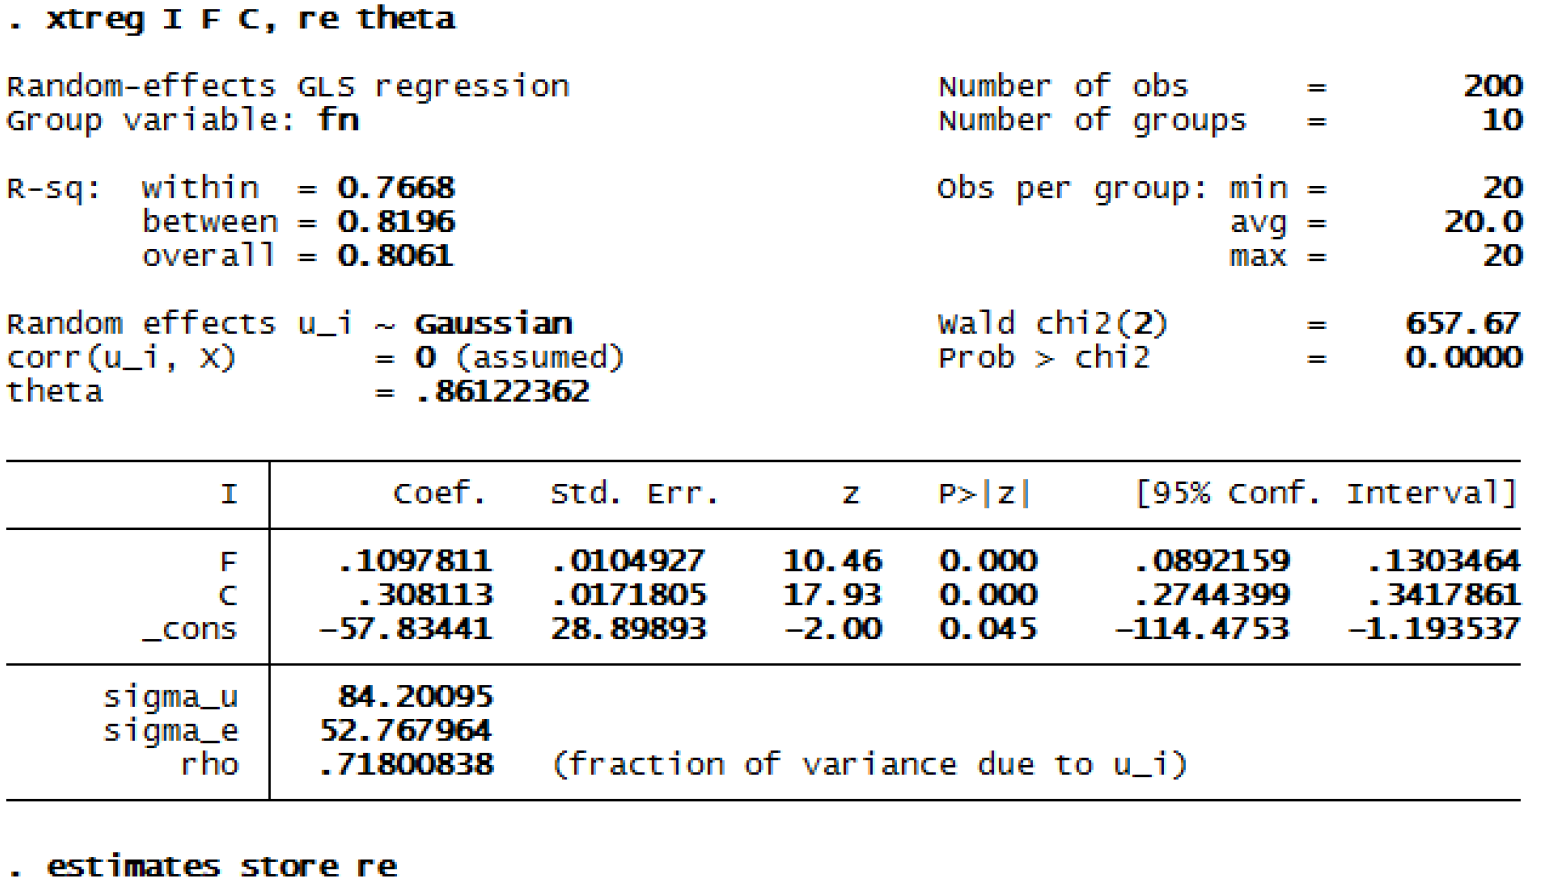
\includegraphics[width = 0.85\linewidth]{figures/panel_07.png}
		\end{figure}
\end{frame}
%------------------------------------------------
\begin{frame}{Random-Effect (RE) options}
		\begin{figure}
			\centering
			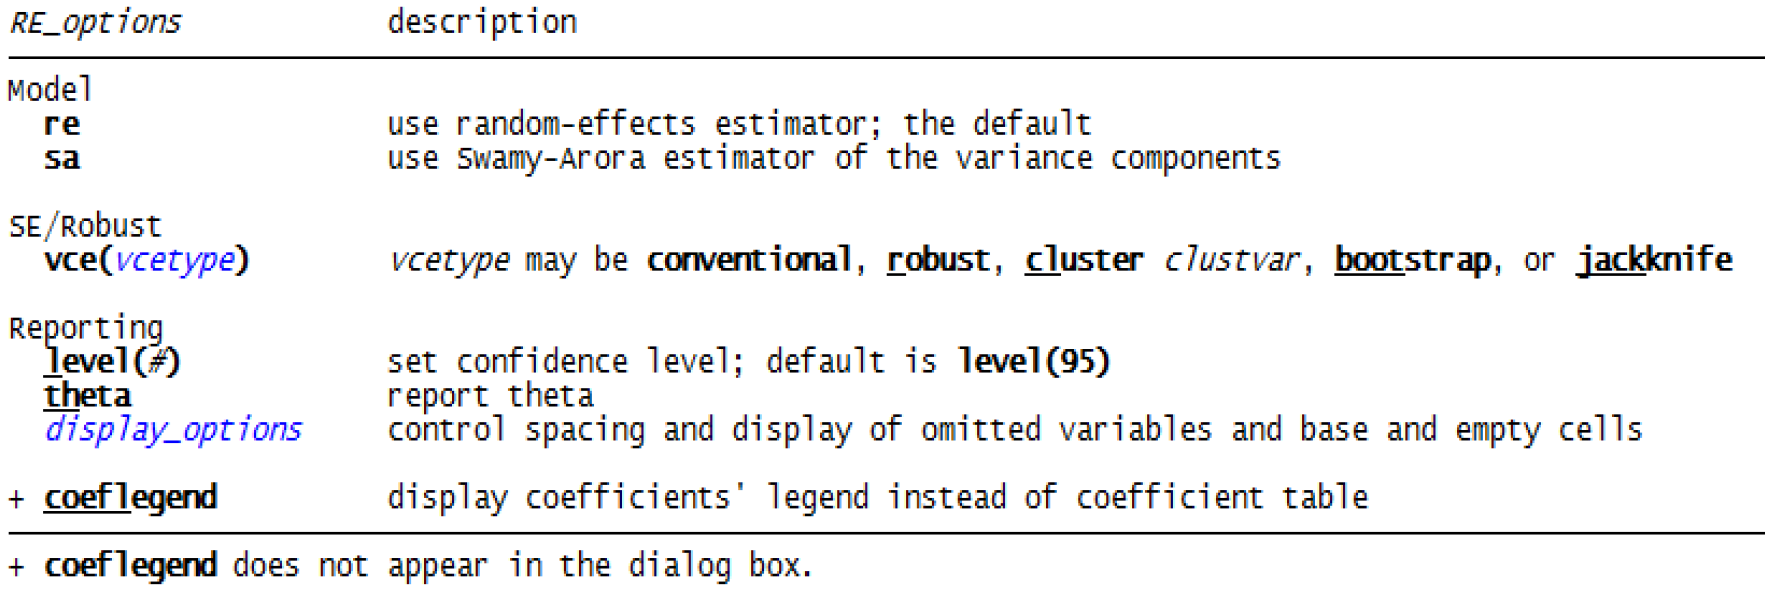
\includegraphics[width = \linewidth]{figures/panel_08.png}
		\end{figure}
\end{frame}
%------------------------------------------------
\begin{frame}{FGLS strategy: MLE iterative}	
	Breusch (1987) concentrates the likelihood with respect to:%
			$$\widehat{\phi }^{2}=\frac{d^{\prime }Qd}{\left( T-1\right) d^{\prime }\left(
				P-\overline{J}_{NT}\right) d}=\frac{\sum_{i=1}^{N}\sum_{t=1}^{T}\left(
				d_{it}-\overline{d}_{i}\right) ^{2}}{T\left( T-1\right) \sum_{i=1}^{N}\left( 
				\overline{d_{i\cdot }}-\overline{d}_{\cdot \cdot }\right) ^{2}}$$
	where $d=y-X\widehat{\beta }$, and $\phi ^{2}=\frac{\sigma _{\nu }^{2}}{\sigma _{1}^{2}},$ in fact $\theta \backsim 1-\phi $
		\begin{align*}
			\widehat{\beta }_{mle} = & \left[X^{\prime}\left(Q+\phi^{2}\left(P-
									   \overline{J}_{NT}\right) \right) X\right] ^{-1} \\
									 & \left[X^{\prime}\left(Q+\phi^{2}\left(P-\overline{J}_{NT}\right)
									   \right)y\right]^{-1}
		\end{align*}
	iteration process in order to get $\widehat{\beta}_{mle}.$ be careful of values $\phi$ this should be positive and finite.
\end{frame}
%------------------------------------------------
\begin{frame}{MLE iterative STATA syntax}
		\begin{figure}
			\centering
			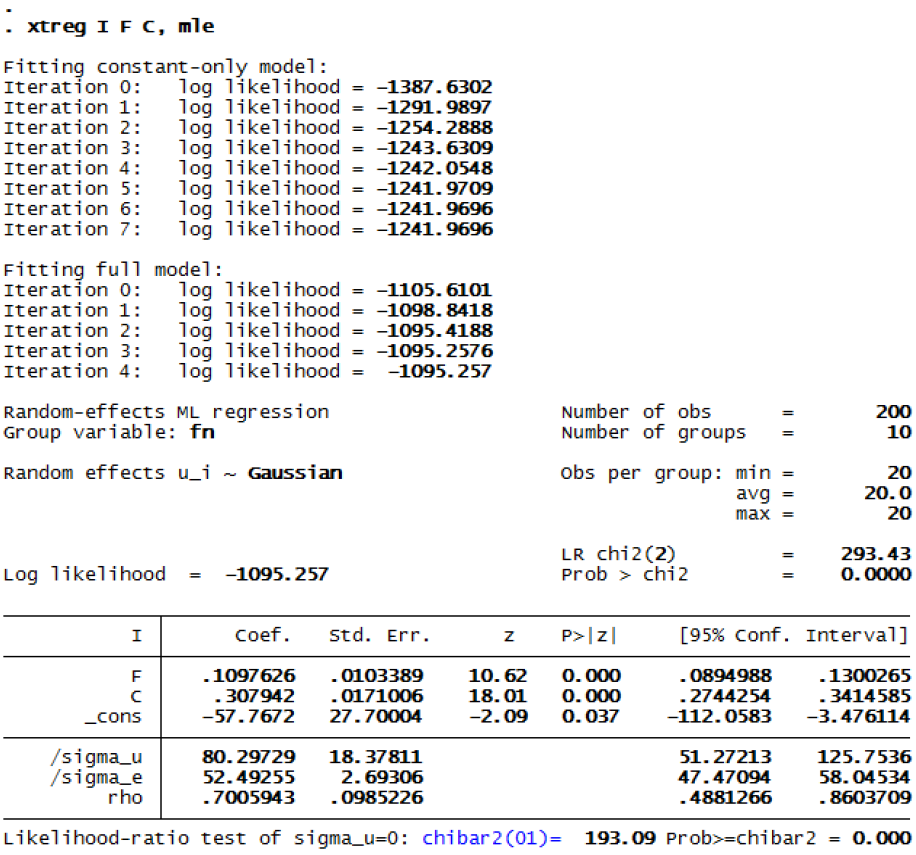
\includegraphics[width = 0.5\linewidth]{figures/panel_09.png}
		\end{figure}
\end{frame}
%------------------------------------------------
\begin{frame}{Interpretation of Phi}
	\begin{itemize}
		\item if $\phi =0\Rightarrow $ within-group estimator
		\item if $\phi =\infty \Rightarrow $ between-group estimator
	\end{itemize}
\end{frame}

%------------------------------------------------------------------------------------
\subsection{Estimating in STATA}
%------------------------------------------------------------------------------------

\begin{frame}{Estimating in STATA}
	\begin{center}
		\Huge{Let's go to STATA!}
	\end{center}
\end{frame}

\begin{frame}{Summarizing the STATA results}
		\begin{figure}
			\centering
			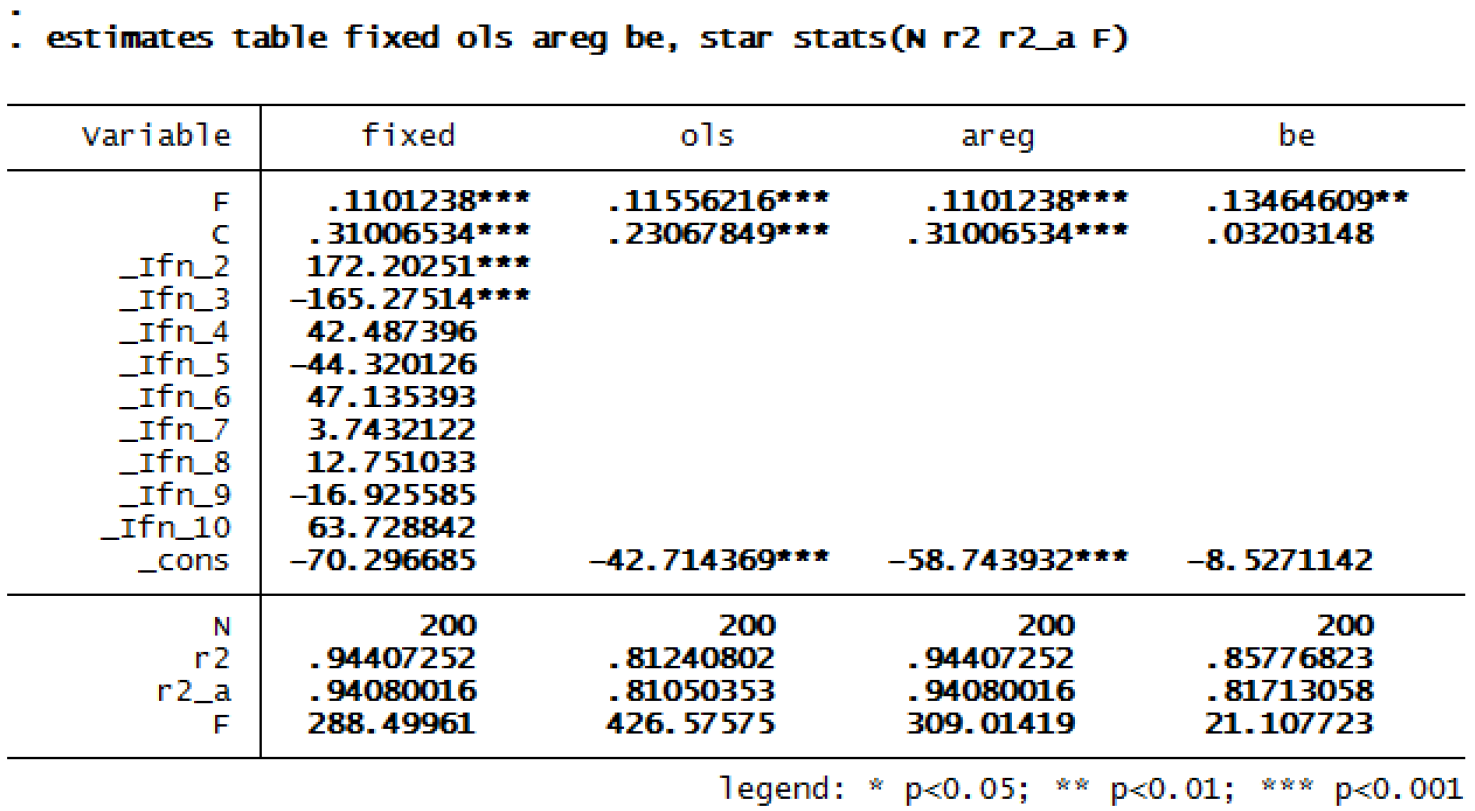
\includegraphics[width = 0.9\linewidth]{figures/panel_stata_01.png}
		\end{figure}
\end{frame}

\begin{frame}{Summarizing the STATA results}
		\begin{figure}
			\centering
			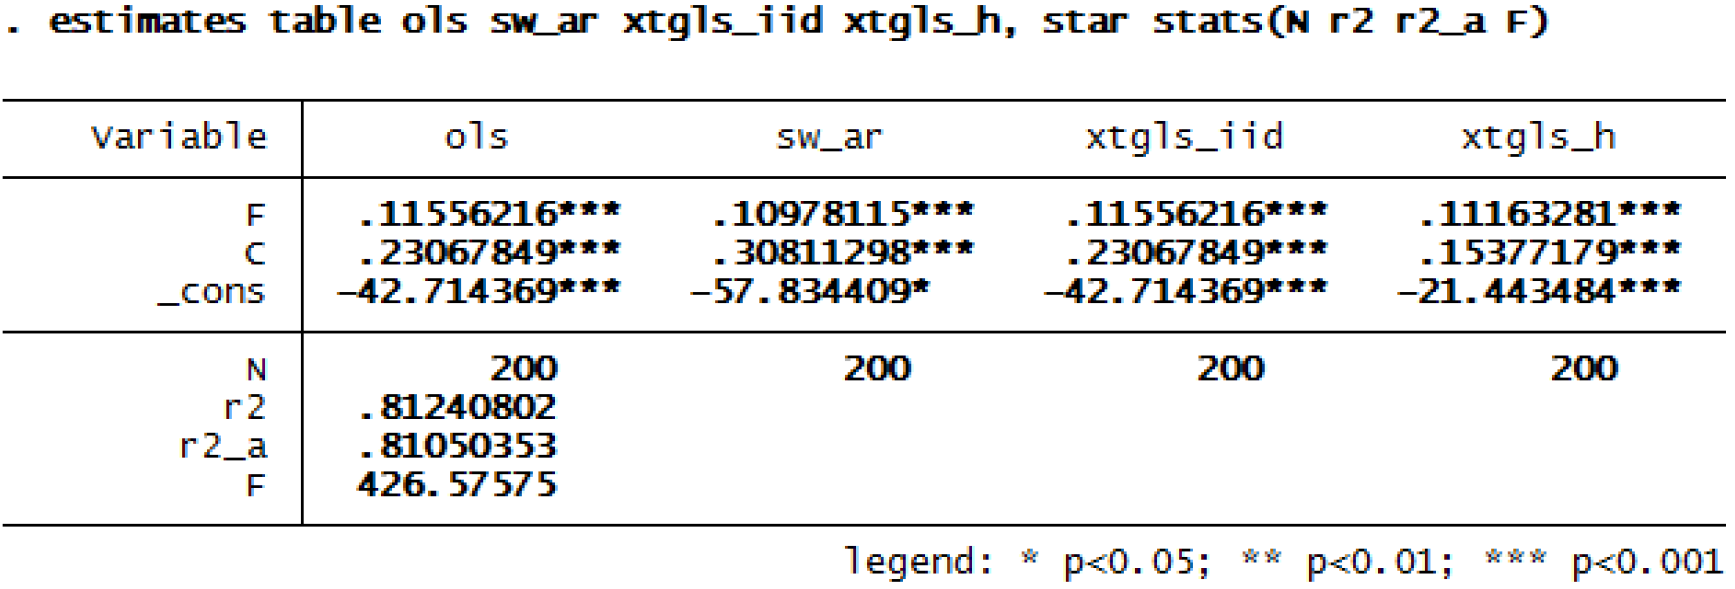
\includegraphics[width = \linewidth]{figures/panel_stata_02.png}
		\end{figure}
\end{frame}

\begin{frame}{Summarizing the STATA results}
		\begin{figure}
			\centering
			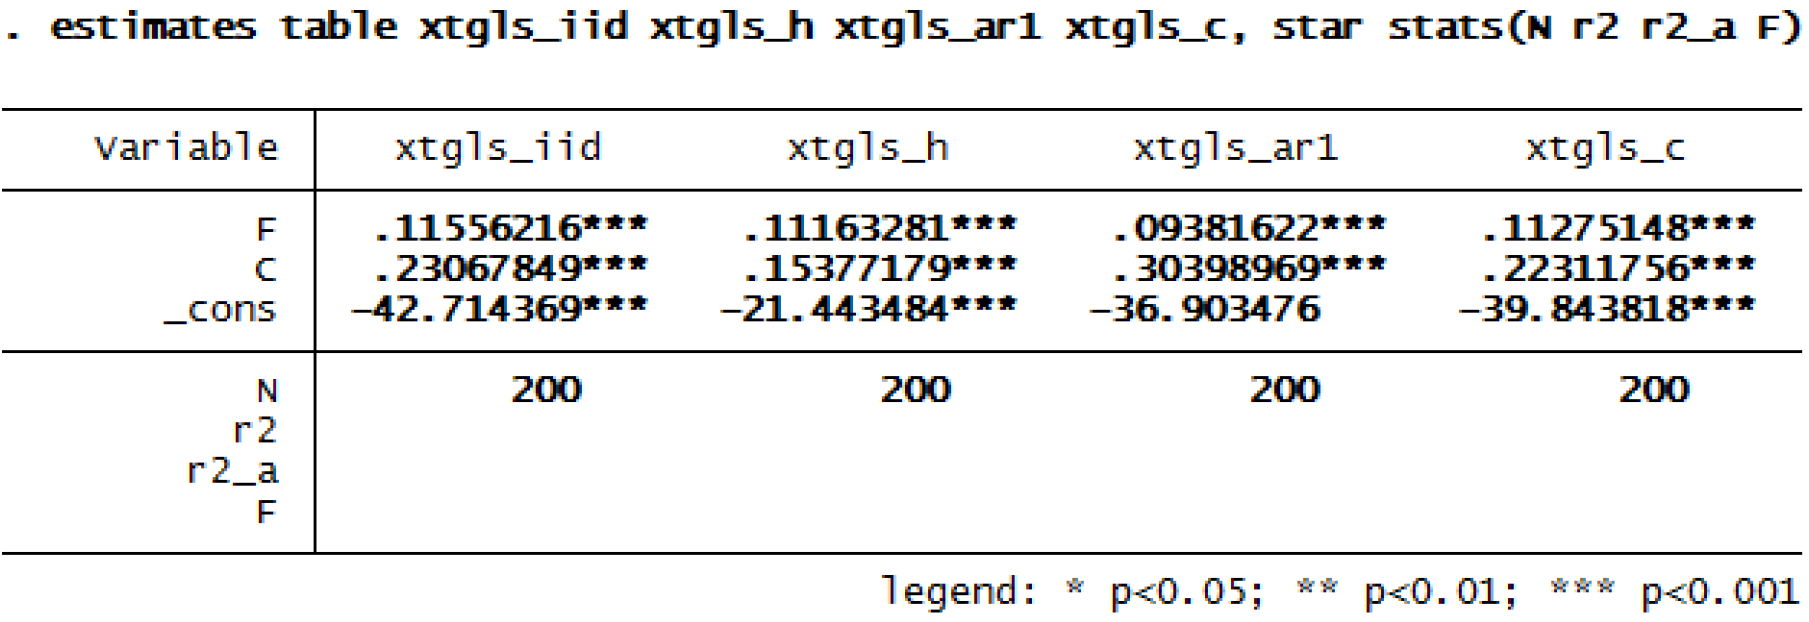
\includegraphics[width = \linewidth]{figures/panel_stata_03.png}
		\end{figure}
\end{frame}